%%
%% This is a skeleton file demonstrating the use of IEEEtran.cls
%% (requires IEEEtran.cls version 1.8a or later) with an IEEE
%% Computer Society journal paper.
%%
%% Support sites:
%% http://www.michaelshell.org/tex/ieeetran/
%% http://www.ctan.org/tex-archive/macros/latex/contrib/IEEEtran/
%% and
%% http://www.ieee.org/
%%
%% bare_jrnl_compsoc.tex
%% V1.4a
%% 2014/09/17
%% by Michael Shell
%% See:
%% http://www.michaelshell.org/
%% for current contact information.

\documentclass[10pt,journal,compsoc]{IEEEtran}


% *** CITATION PACKAGES ***
%
\ifCLASSOPTIONcompsoc
  % IEEE Computer Society needs nocompress option
  % requires cite.sty v4.0 or later (November 2003)
  \usepackage[nocompress]{cite}
\else
  % normal IEEE
  \usepackage{cite}
\fi
% cite.sty was written by Donald Arseneau




% *** GRAPHICS RELATED PACKAGES ***
%
\ifCLASSINFOpdf
  \usepackage[pdftex]{graphicx}
   \graphicspath{{figures/}}
  % declare the path(s) where your graphic files are
  % \graphicspath{{../pdf/}{../jpeg/}}
  % and their extensions so you won't have to specify these with
  % every instance of \includegraphics
  % \DeclareGraphicsExtensions{.pdf,.jpeg,.png}
\else
  % or other class option (dvipsone, dvipdf, if not using dvips). graphicx
  % will default to the driver specified in the system graphics.cfg if no
  % driver is specified.
  % \usepackage[dvips]{graphicx}
  % declare the path(s) where your graphic files are
  % \graphicspath{{../eps/}}
  % and their extensions so you won't have to specify these with
  % every instance of \includegraphics
  % \DeclareGraphicsExtensions{.eps}
\fi
% graphicx was written by David Carlisle and Sebastian Rahtz.


% *** MATH PACKAGES ***
%
\usepackage[cmex10]{amsmath}
% A popular package from the American Mathematical Society that provides
% many useful and powerful commands for dealing with mathematics.

\usepackage{amsfonts} % to use $\mathbb{Z}$


% *** SPECIALIZED LIST PACKAGES ***
\usepackage{algorithm}
\usepackage{algorithmic}
% algorithmic.sty was written by Peter Williams and Rogerio Brito.


% *** ALIGNMENT PACKAGES ***
%
%\usepackage{array}
% Frank Mittelbach's and David Carlisle's array.sty patches and improves
% the standard LaTeX2e array and tabular environments to provide better
% appearance and additional user controls.




% correct bad hyphenation here
\hyphenation{op-tical net-works semi-conduc-tor}


\begin{document}

\title{Bare Demo of IEEEtran.cls\\ for Computer Society Journals}
\author{Miguel P. Xochicale
%\thanks{Manuscript received April 19, 2005; revised September 17, 2014.}
}


% The paper headers
\markboth{Template for manuscripts, 9th~October~2015}%
{Shell \MakeLowercase{\textit{et al.}}: Bare Demo of IEEEtran.cls for Computer
Society Journals}
% The only time the second header will appear is for the odd numbered pages
% after the title page when using the twoside option.
%
% *** Note that you probably will NOT want to include the author's ***
% *** name in the headers of peer review papers.                   ***
% You can use \ifCLASSOPTIONpeerreview for conditional compilation here if
% you desire.



% The publisher's ID mark at the bottom of the page is less important with
% Computer Society journal papers as those publications place the marks
% outside of the main text columns and, therefore, unlike regular IEEE
% journals, the available text space is not reduced by their presence.
% If you want to put a publisher's ID mark on the page you can do it like
% this:
%\IEEEpubid{0000--0000/00\$00.00~\copyright~2014 IEEE}
% or like this to get the Computer Society new two part style.
%\IEEEpubid{\makebox[\columnwidth]{\hfill 0000--0000/00/\$00.00~\copyright~2014 IEEE}%
%\hspace{\columnsep}\makebox[\columnwidth]{Published by the IEEE Computer Society\hfill}}
% Remember, if you use this you must call \IEEEpubidadjcol in the second
% column for its text to clear the IEEEpubid mark (Computer Society jorunal
% papers don't need this extra clearance.)


% use for special paper notices
%\IEEEspecialpapernotice{(Invited Paper)}


% for Computer Society papers, we must declare the abstract and index terms
% PRIOR to the title within the \IEEEtitleabstractindextext IEEEtran
% command as these need to go into the title area created by \maketitle.
% As a general rule, do not put math, special symbols or citations
% in the abstract or keywords.
\IEEEtitleabstractindextext{%

\begin{abstract}
 The following template is considered for future submission of my research. I believe that
 any advance in  science should be freely released in order that anyone
 who is interested in the idea can reproduce the current advances.
 To share, to modify and to improve are the bacis principles for pushing the
 the boundaries of any discipline in science.
\end{abstract}

% Note that keywords are not normally used for peerreview papers.
\begin{IEEEkeywords}
Activity Recognition; On-Body Inertial Sensors; Motor Skill Assessment; Human-Robot Interaction
\end{IEEEkeywords}}


% make the title area
\maketitle


% To allow for easy dual compilation without having to reenter the
% abstract/keywords data, the \IEEEtitleabstractindextext text will
% not be used in maketitle, but will appear (i.e., to be "transported")
% here as \IEEEdisplaynontitleabstractindextext when the compsoc
% or transmag modes are not selected <OR> if conference mode is selected
% - because all conference papers position the abstract like regular
% papers do.
\IEEEdisplaynontitleabstractindextext
% \IEEEdisplaynontitleabstractindextext has no effect when using
% compsoc or transmag under a non-conference mode.



% For peer review papers, you can put extra information on the cover
% page as needed:
% \ifCLASSOPTIONpeerreview
% \begin{center} \bfseries EDICS Category: 3-BBND \end{center}
% \fi
%
% For peerreview papers, this IEEEtran command inserts a page break and
% creates the second title. It will be ignored for other modes.
\IEEEpeerreviewmaketitle



\IEEEraisesectionheading{\section{Introduction}\label{sec:introduction}}
% Computer Society journal (but not conference!) papers do something unusual
% with the very first section heading (almost always called "Introduction").
% They place it ABOVE the main text! IEEEtran.cls does not automatically do
% this for you, but you can achieve this effect with the provided
% \IEEEraisesectionheading{} command. Note the need to keep any \label that
% is to refer to the section immediately after \section in the above as
% \IEEEraisesectionheading puts \section within a raised box.

% The very first letter is a 2 line initial drop letter followed
% by the rest of the first word in caps (small caps for compsoc).
%
% form to use if the first word consists of a single letter:
% \IEEEPARstart{A}{demo} file is ....
%
% form to use if you need the single drop letter followed by
% normal text (unknown if ever used by IEEE):
% \IEEEPARstart{A}{}demo file is ....
%
% Some journals put the first two words in caps:
% \IEEEPARstart{T}{his demo} file is ....
%
% Here we have the typical use of a "T" for an initial drop letter
% and "HIS" in caps to complete the first word.


\IEEEPARstart{A}{ccording} to Bulling \emph{et al.}  \cite{bulling2014} the common challenges in
HAR using body-worn sensors are:
(i) \textit{intraclass variability} which occurs when an activity is performed differently
either by a single person or several people. For example, gait patterns may be more
dynamic in the morning after sleep than in the evening after a day full of activities;
(ii) \textit{interclass similarity} occurs when the sensor data is very similar. For example,
in recognising dietary activity, drinking water or coffee entails the same arm movements
\cite{amft2008phd};
and (iii) \textit{the NULL class problem} occurs
when ambiguous activities are irrelevant for the recognition methods
which leads to wrong classification of the activities \cite{amft2011}.
Recently, Bulling \emph{et al.}  \cite{bulling2014} reviewed advances in
the Activity Recognition Chain (ARC) using body-worn sensors.
The general ARC comprehend five stages (data acquisition, signal preprocessing,
segmentation, feature extraction and selection training and classification) of which
the applied technique in each stage depends on the activity to recognise.

Given the case of the variability in dance activities, it is hypothesised that
there are three possible reasons for variation:
(i) inherent noise in body-worn sensors,
(ii) inherent properties of the activity itself and
(iii) differences in the people performing the activity,
e.g., gender, anthropometry or level of skills.

\subsection{Research Questions}

For this PhD, the time-delay embedding and PCA methods
have proven to be a reliable method
for feature extraction in HAR \cite{Frank2010, Sama2013},
it is therefore hypothesised that these methods might be suitable
to learn the variability of human activities.
Therefore, the following research questions will be addressed:
\begin{enumerate}
 \item In the light of limitations of time-delay embedding and PCA,
 which other non-linear analysis tools would be suitable to explore
\item The variability in different human activities and use them as a features
 for machine learning algorithms?


\end{enumerate}


\section{Time-Delay Embedding}
The aim of the time-delay embedding, also known as Takens Theorem \cite{Takens1981},
is to reconstruct a $k-$dimensional manifold $M$ of an unknown dynamical system $s(t)$
from a time series $x(t)$ with discrete observations at given time points $t$.
Time-delay embedding assumes that the time series
is a sequence $x(t)=h[s(t)]$,  where  $h: M \rightarrow \mathbb{R}$
is a measurement function in the unknown dynamical system, being $x(t)$ measurable.

Thus, the time delay reconstruction is defined as:
$\overline{x}(t) = (x(t), x(t-\tau),...,x(t-(m-1)\tau))$
where $m$ is the embedding dimension and $\tau$ is the embedding time-delay.
$\overline{x}(t)$ defines a map $\varPhi: M \rightarrow \mathbb{R}^m$ such that
$\overline{x}(t) = \varPhi(s)$.
Similarly, $y(t)= \varPsi [\overline{x}(t)]$ is a $n$-dimensional vector
where $\varPsi: \mathbb{R}^m \rightarrow \mathbb{R}^n$ is a further transformation.
Figure \ref{fig:takenstheorem} illustrate the time delay reconstruction process.
For details, see the work of Uzal \emph{et al.} \cite{Uzal2011}.

\begin{figure}[!htb]
\centering
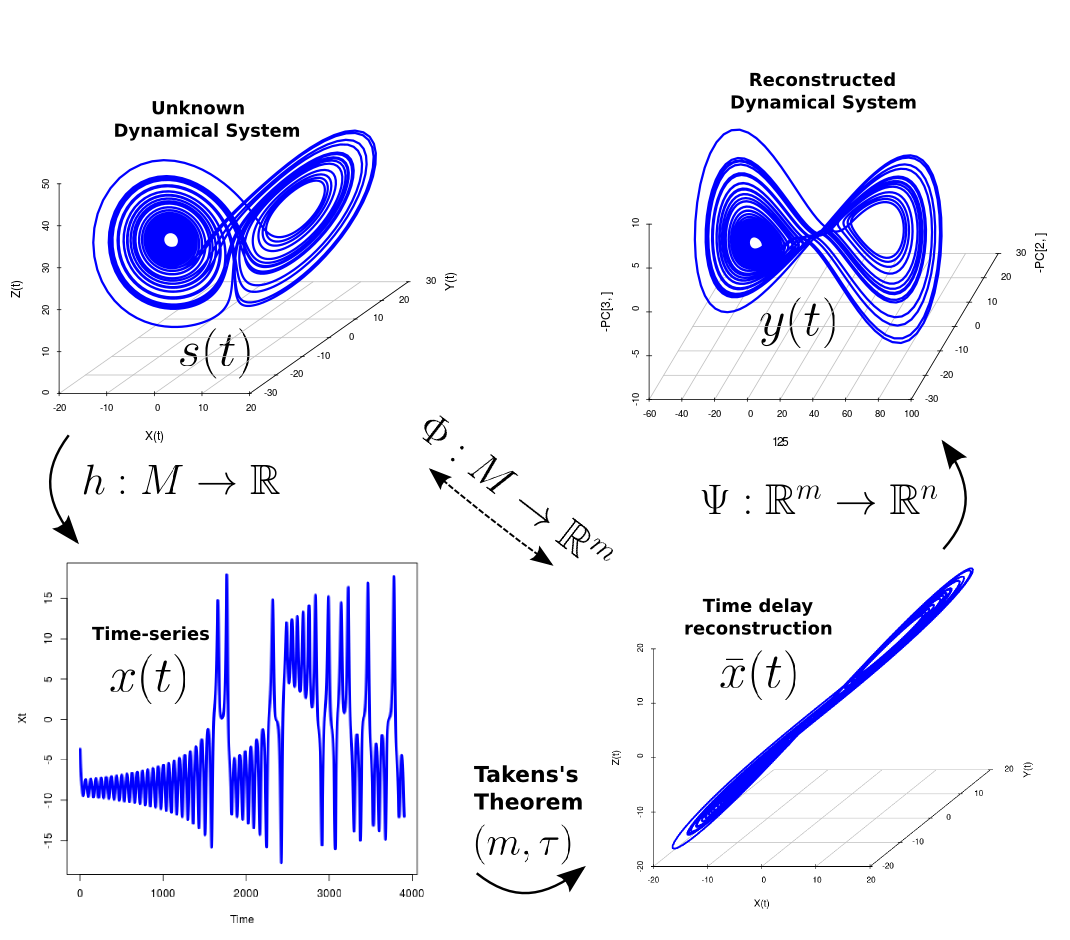
\includegraphics[width=0.45\textwidth]{takenstheorem}
\caption[PA]{The reconstruction problem. The figure is based on the work of Uzal
\emph{et al.} \cite{Uzal2011}.}
\label{fig:takenstheorem}
\end{figure}

\subsection{Embedding Parameters $m$ and $\tau$}
Given any time series $x(t)$, the time delay reconstruction system, $\overline{x}(t)$,
is easy to implement. For this work, Cao's method \cite{Cao1997}, a modification of the
False Nearest Neighbours (FNN) algorithm, and mutual information algorithm by

\subsubsection{Minimum Embedding Dimension $m_{min}$}
Cao's method \cite{Cao1997} for computing the minimal embedding dimension is based on
the mean values $E1(d)$ and $E2(d)$ in which $d$ is a given embedding dimension value.

$E1(d)$ is used to obtain the minimal dimension $m_{min}$ and stops changing
when the time series comes from an attractor.
We computed $E1(d)$ values for $1 \leq \tau \leq 10$ to exemplify
the minor dependency of $\tau$ given periodic, chaotic and random time series.

The second of these values, $E2(d)$, is used to distinguish
deterministic signals from random signals in which case the $E2(d)$ values will be approximately
equal to 1 for any $d$.
Similarly, we computed $E2(d)$ values for periodic, chaotic and random time series,
to exemplify the no significant dependency on $\tau$, where $1 \leq \tau \leq 10$.

Cao's method is a modified version of the FNN method, and $E1(d)$ and
$E2(d)$ values are only dependant on $m$ and $\tau$ \cite{Cao1997}.

\subsubsection{Minimum Time-delay Embedding  $\tau_{min}$}
The method of choosing the minimum Time-delay embedding, $\tau_{min}$, was proposed
by Fraser \emph{et al.}  in which the first minimum of the mutual
information graph is chosen to estimate the minimal time-delay embedding parameter.
The local minimum for the Chaotic series is $\tau_{min} = 18$.
On the other hand, for random time series the mutual information plot have no local minimum
and values are monotonically decreasing which means that $\tau_{min} = 1$.
However, further research has to be done when data comes from a periodic time series
since its minimum in the mutual information plot appears to be at $\tau_{min} = 3$.

\section{The Activity Recognition Chain}

Bulling \emph{et al.} \cite{bulling2014} reviewed the state of the art of
HAR using body-worn inertial sensors.

The first stage of the ARC is the raw data collection from several sensors attached to
different parts of the body. Sensors data over a given time, $s_i$, provide multiple values  $d^i$,
(e.g. $d^1, d^2, d^3$ for 3-D acceleration referred to as x, y and z direction)
\begin{equation}
s_i = (\textbf{d}^1, \textbf{d}^2,\dots \textbf{d}^t) \mbox{,for } i=1, \dots,k
\end{equation}
where $k$ denotes the number of sensors.

In the preprocessing stage of the ARC, raw multivariable time series are transformed into a
pre-processed time series $D'= (d'_1, \dots, d'_n )^T$, where $d'_i$ is one dimension
of the data for the preprocessed time series and $n$ is the number of total data dimensions.
Different methods for the preprocessing tasks may be applied to the raw data
(e.g. synchronisation, calibration, unit conversion, normalisation, resampling, denoising
or baseline drift removal \cite{bulling2014}).

The stage of data segmentation identifies segments within the continuous data stream
that are likely to have information about activities. The segmentation stage creates
a set of segments $w_m$ % containing a possible activity $y$
such that
\begin{equation}
W = \{   w_1, \dots, w_m  \},
\end{equation}
where $m$ correspond to the number of segments.
Since the segmentation of the data is a difficult problem, there are various methods
in the literature to tackle this problem: sliding window, energy-based segmentation,
rest-position segmentation, additional sensors and external context sources.

In the feature extraction stage, a feature extraction function $F$ reduces
the signals $D'$  into segmented signals $W$.
The total number of features $X_i$ is the feature space.
\begin{equation}
X_i = F ( D', w_i)
\end{equation}
In the literature on activity recognition, different  methods for feature extraction
can be found including signal-based features, body model features, event-based features,
multilevel features or automatic feature ranking and selection.

Machine learning tools have been used in HAR over the last 15 years
so as to describe, analyse and predict human activities \cite{bulling2014}.
However, the chosen approach is subject to computational complexity,
recognition performance or latency.
Generally for the learning stage, a training data set $T = \{ X_i, y_i \}  ^N _ {i=1}$
is computed prior to the classification with $N$ pairs of feature vectors $X_i$ and ground
truth labels $y^i$ (possible activities to recognise). For this stage, model parameters
$\theta$ can be learned to decrease the classification error on $T$.
Then, with the trained model $T$, each feature vector $X_i$  is mapped to a set of class labels
$Y= \{ y^1, \dots , y^c \}$ with scores $P_i = \{ p^1_i, \dots, p^c_i \}$:
\begin{equation}
p_i ( y \mid X_i, \theta) = I (X_i, \theta) \mbox{,for } y \in Y
\end{equation}
and inference method $I$.
Finally, the classification output $y_i$ is computed with the maximum score $P_i$
\begin{equation}
y_i  =
\underset{ y \in Y, p \in P_i }{\text{argmax}}   p(y | X_i, \theta)
\end{equation}
The most common classification algorithms are: decision trees, Bayesian models,
domain transform, fuzzy logic, Markov models, support vector machines (SVM),
artificial neural networks (ANN) and ensembles of classifiers \cite{Lara2013}.

Similarly, when the recognition of activities can miss, confuse or falsely
recognise activities that did occur, several metrics
can be used to optimise the classification. Some of the metrics
are confusion matrices, accuracy, precision, recall, and F-scores,
decision-independent Precision-Recall or receiver operating characteristic
curves (ROC curves) \cite{bulling2014}.


\section{Artificial Signals}
To understand the possible sources of variability
in dance activities, I followed the method of Hammerla
\emph{et al.} \cite{hammerla2011} which might be useful to model:
i) noise in sensors,
ii) properties of activities and
iii) properties of people.

The proposal of Hammerla \emph{et al.} \cite{hammerla2011}
is aimed to examine the effects of
variability in the precision of motion  (additive noise)
and in the strategy of motion  (structural noise) of
activities using artificial signals.

Additive noise is normalised noise with variance $\sigma_a ^2$ added to the
sinusoid signal $S$:
\begin{equation}
 S^a = S + \textbf{N}(0, \sigma_a ^2)
\end{equation}

Structural noise is a sinusoid signal distorted with different variance
in frequency and amplitude $\sigma_s ^2$ and window length $w_s$.
Algorithm 1 describes the creation of structural noise.
To make the data less redundant for possible variations of environmental
conditions or body-worn sensor mobility in users, the data is whitened
(i.e. data is normalised to have zero mean and unit variance)


% http://tex.stackexchange.com/questions/219816/algorithm-in-ieee-format
\begin{algorithm}[H]
\caption{Structural Noise}
\begin{algorithmic}[1]
 \renewcommand{\algorithmicrequire}{\textbf{Input:}}
 \renewcommand{\algorithmicensure}{\textbf{Output:}}
 \REQUIRE time-series $S^a$, variance $\sigma_s ^2$, window length $w_s$
 \ENSURE  Structurally distorted signal $S^s$
  \FOR {$j = 1$ to $L$, $j=j+w_s$}
  \STATE $\textbf{u'} \leftarrow \textbf{N}(0, \sigma_s ^2)$
  \STATE $S^{a} =$ sinusoid with frequency $| \textbf{u'} |$ and variance $\sigma_a ^2$ of length $w_s$
  \STATE $S^s_{j \rightarrow j+w_s}  = S^s_{j \rightarrow j+w_s}  + S^{a} \times   \sigma_s ^2 $
  \ENDFOR
  \\ $S^s= whiten (S^s)$
 \RETURN $S^s$
\end{algorithmic}
\end{algorithm}

By varying both $\sigma_a ^2$ and $\sigma_s ^2$,
it is possible to simulate and control the additive noise and the structural noise
in the structure of the human activity. For example, low values of $\sigma_a ^2$
are associated with precise movements while low values of $\sigma_s ^2$ correspond
to a well chosen strategy for a motion.



\section{Future Work}
To raise the bar in the field of human activity recognition,
the plan for the next six months is:

\begin{itemize}
\item \textbf{Sep. 2015 (11th)}  Using the sawing data, present the limitations of
    time-delay embedding and PCA and propose improvements for the method.
    I am also planning to investigate other non-linear analysis tools that would be suitable
	to explore the variability of dance activities.
 \item \textbf{Oct. 2015 (12th)} Work towards a submission in Measuring Behavior 2016 and Augmented Human 2016 conferences.
 \item \textbf{Nov. 2015 (13th)} Submit works in the Measuring Behavior 2016 and Augmented Human 2016 conferences.
 \item \textbf{Dec. 2015 (14th)} Search for an appropriate journal and work towards a submission.
 \item \textbf{Jan. 2016 (15th)} Submit a journal publication
\end{itemize}


% use section* for acknowledgment
\ifCLASSOPTIONcompsoc
  % The Computer Society usually uses the plural form
  \section*{Acknowledgments}
\else
  % regular IEEE prefers the singular form
  \section*{Acknowledgment}
\fi

Miguel Perez-Xochicale gratefully acknowledges the studentship from
the National Council for Science and Technology (CONACyT) Mexico
from November 2014 to November 2017 to pursue his postgraduate studies
at University of Birmingham.

% Can use something like this to put references on a page
% by themselves when using endfloat and the captionsoff option.
\ifCLASSOPTIONcaptionsoff
  \newpage
\fi


% trigger a \newpage just before the given reference
% number - used to balance the columns on the last page
% adjust value as needed - may need to be readjusted if
% the document is modified later
%\IEEEtriggeratref{8}
% The "triggered" command can be changed if desired:
%\IEEEtriggercmd{\enlargethispage{-5in}}

% references section

% can use a bibliography generated by BibTeX as a .bbl file
% BibTeX documentation can be easily obtained at:
% http://www.ctan.org/tex-archive/biblio/bibtex/contrib/doc/
% The IEEEtran BibTeX style support page is at:
% http://www.michaelshell.org/tex/ieeetran/bibtex/
%\bibliographystyle{IEEEtran}
% argument is your BibTeX string definitions and bibliography database(s)
%\bibliography{IEEEabrv,../bib/paper}
%
% <OR> manually copy in the resultant .bbl file
% set second argument of \begin to the number of references
% (used to reserve space for the reference number labels box)
% \begin{thebibliography}{1}
%
% \bibitem{IEEEhowto:kopka}
% H.~Kopka and P.~W. Daly, \emph{A Guide to \LaTeX}, 3rd~ed.\hskip 1em plus
%   0.5em minus 0.4em\relax Harlow, England: Addison-Wesley, 1999.
%
% \end{thebibliography}

% \nocite{*}
\bibliographystyle{IEEEtran}
\bibliography{references}


% biography section
%
% If you have an EPS/PDF photo (graphicx package needed) extra braces are
% needed around the contents of the optional argument to biography to prevent
% the LaTeX parser from getting confused when it sees the complicated
% \includegraphics command within an optional argument. (You could create
% your own custom macro containing the \includegraphics command to make things
% simpler here.)
%\begin{IEEEbiography}[{\includegraphics[width=1in,height=1.25in,clip,keepaspectratio]{mshell}}]{Michael Shell}
% or if you just want to reserve a space for a photo:

% \begin{IEEEbiography}[{\includegraphics[width=1in,height=1.25in,clip,keepaspectratio]{mxochicale38x44.pdf}}]{name}

% \begin{IEEEbiography}{Miguel Perez-Xochicale}
% ........................
% \end{IEEEbiography}



% % if you will not have a photo at all:
% \begin{IEEEbiographynophoto}{John Doe}
% Biography text here.
% \end{IEEEbiographynophoto}
%
% % insert where needed to balance the two columns on the last page with
% % biographies
% %\newpage
%
% \begin{IEEEbiographynophoto}{Jane Doe}
% Biography text here.
% \end{IEEEbiographynophoto}

% You can push biographies down or up by placing
% a \vfill before or after them. The appropriate
% use of \vfill depends on what kind of text is
% on the last page and whether or not the columns
% are being equalized.

%\vfill

% Can be used to pull up biographies so that the bottom of the last one
% is flush with the other column.
%\enlargethispage{-5in}



% that's all folks
\end{document}
